%------------------------------------------------------------------------------------
% A comentar
%------------------------------------------------------------------------------------
% \documentclass[a4paper,11pt]{book} % Fonte do livro
% %----------------------------------------------------------------------------------
% The Legrand Orange Book
% Structural Definitions File
% Version 2.0 (9/2/15)
%----------------------------------------------------------------------------------
% \documentclass[a4paper,11pt]{book} % Fonte do livro

%----------------------------------------------------------------------------------
%	VARIOUS REQUIRED PACKAGES AND CONFIGURATIONS
%----------------------------------------------------------------------------------
\usepackage[top=3cm,bottom=3cm,left=3cm,right=2cm,headsep=10pt,a4paper]{geometry} % Page margins
\usepackage{import}
\usepackage{lipsum} % Inserts dummy text
\usepackage[brazil]{babel} % Brazil language/hyphenation
\usepackage{graphicx} % Required for including pictures
\usepackage{wrapfig} % Imagens que se cruzam com texto
\usepackage{tikz} % Required for drawing custom shapes
\usepackage[T1]{fontenc}
\usepackage[utf8]{inputenc} % Required for including letters with accents
\usepackage{enumitem} % Customize lists
\usepackage{longtable}
\usepackage{booktabs} % Required for nicer horizontal rules in tables
\usepackage{xcolor} % Required for specifying colors by name
\usepackage{listings} % listagens
\usepackage{float}
%----------------------------------------------------------------------------------
%	IMAGENS
%----------------------------------------------------------------------------------
\graphicspath{{Pictures/}} % Specifies the directory where pictures are stored
%----------------------------------------------------------------------------------
%	CAIXA DE LISTAGEM
%----------------------------------------------------------------------------------
\definecolor{ocre}{RGB}{243,102,25} % Define the orange color used for highlighting throughout the book
% Definição para as caixas de listagens
\definecolor{codegray}{rgb}{0.5,0.5,0.5}
\definecolor{backcolour}{rgb}{0.95,0.95,0.92}

% Espaçamento dos Parágrafos
\setlength{\parindent}{0em}
\setlength{\parskip}{1em}

\lstset {
 aboveskip=3mm,
 backgroundcolor=\color{backcolour},
 basicstyle={\small\ttfamily},
 belowskip=3mm,
 breaklines=true,
 breakatwhitespace=true,
 columns=flexible,
 commentstyle=\textit,
 frame=tb,
 keepspaces=true,
 keywordstyle=\color{blue}\bfseries,
 % language=Java, Python, HTML, CSS
 showstringspaces=false,
 showtabs=false,
 tabsize=3
}
%----------------------------------------------------------------------------------
%	FONTS
%----------------------------------------------------------------------------------
\usepackage{avant} % Use the Avantgarde font for headings
\usepackage{mathptmx} % Use the Adobe Times Roman as the default text font together
\usepackage{microtype} % Slightly tweak font spacing for aesthetics
\usepackage[T1]{fontenc} % Use 8-bit encoding that has 256 glyphs
%----------------------------------------------------------------------------------
%	BIBLIOGRAPHY AND INDEX
%----------------------------------------------------------------------------------
% \usepackage[style=numeric,citestyle=numeric,sorting=nyt,sortcites=true,autopunct=true,hyperref=true,abbreviate=false,backref=true,backend=biber]{biblatex}
%\addbibresource{bibliography.bib} % BibTeX bibliography file
% \defbibheading{bibempty}{}
\usepackage{calc} % For simpler calculation - used for spacing the index letter headings correctly
\usepackage{makeidx} % Required to make an index
\makeindex % Tells LaTeX to create the files required for indexing
%----------------------------------------------------------------------------------
%	MAIN TABLE OF CONTENTS
%----------------------------------------------------------------------------------
\usepackage{titletoc} % Required for manipulating the table of contents
\contentsmargin{0cm} % Removes the default margin
% Part text styling
\titlecontents{part}[0cm]
{\addvspace{20pt}\centering\large\bfseries}
{}
{}
{}
% Chapter text styling
\titlecontents{chapter}[1.25cm] % Indentation
{\addvspace{12pt}\large\sffamily\bfseries} % Spacing and font options for chapters
{\color{ocre!60}\contentslabel[\Large\thecontentslabel]{1.25cm}\color{ocre}} % Chapter number
{\color{ocre}}  
{\color{ocre!60}\normalsize\;\titlerule*[.5pc]{.}\;\thecontentspage} % Page number
% Section text styling
\titlecontents{section}[1.25cm] % Indentation
{\addvspace{3pt}\sffamily\bfseries} % Spacing and font options for sections
{\contentslabel[\thecontentslabel]{1.25cm}} % Section number
{}
{\hfill\color{black}\thecontentspage} % Page number
[]
% Subsection text styling
\titlecontents{subsection}[1.25cm] % Indentation
{\addvspace{1pt}\sffamily\small} % Spacing and font options for subsections
{\contentslabel[\thecontentslabel]{1.25cm}} % Subsection number
{}
{\ \titlerule*[.5pc]{.}\;\thecontentspage} % Page number
[]
% List of figures
\titlecontents{figure}[0em]
{\addvspace{-5pt}\sffamily}
{\thecontentslabel\hspace*{1em}}
{}
{\ \titlerule*[.5pc]{.}\;\thecontentspage}
[]
% List of tables
\titlecontents{table}[0em]
{\addvspace{-5pt}\sffamily}
{\thecontentslabel\hspace*{1em}}
{}
{\ \titlerule*[.5pc]{.}\;\thecontentspage}
[]
%----------------------------------------------------------------------------------
%	MINI TABLE OF CONTENTS IN PART HEADS
%----------------------------------------------------------------------------------
% Chapter text styling
\titlecontents{lchapter}[0em] % Indenting
{\addvspace{15pt}\large\sffamily\bfseries} % Spacing and font options for chapters
{\color{ocre}\contentslabel[\Large\thecontentslabel]{1.25cm}\color{ocre}} % Chapter number
{}  
{\color{ocre}\normalsize\sffamily\bfseries\;\titlerule*[.5pc]{.}\;\thecontentspage} % Page number
% Section text styling
\titlecontents{lsection}[0em] % Indenting
{\sffamily\small} % Spacing and font options for sections
{\contentslabel[\thecontentslabel]{1.25cm}} % Section number
{}
{}
% Subsection text styling
\titlecontents{lsubsection}[.5em] % Indentation
{\normalfont\footnotesize\sffamily} % Font settings
{}
{}
{}
%----------------------------------------------------------------------------------
%	PAGE HEADERS
%----------------------------------------------------------------------------------
\usepackage{fancyhdr} % Required for header and footer configuration
\pagestyle{fancy}
\renewcommand{\chaptermark}[1]{\markboth{\sffamily\normalsize\bfseries\chaptername\ \thechapter.\ #1}{}} % Chapter text font settings
\renewcommand{\sectionmark}[1]{\markright{\sffamily\normalsize\thesection\hspace{5pt}#1}{}} % Section text font settings
\fancyhf{} \fancyhead[LE,RO]{\sffamily\normalsize\thepage} % Font setting for the page number in the header
\fancyhead[LO]{\rightmark} % Print the nearest section name on the left side of odd pages
\fancyhead[RE]{\leftmark} % Print the current chapter name on the right side of even pages
\renewcommand{\headrulewidth}{0.5pt} % Width of the rule under the header
\addtolength{\headheight}{12pt} % Increase the spacing around the header slightly
\renewcommand{\footrulewidth}{0pt} % Removes the rule in the footer
\fancypagestyle{plain}{\fancyhead{}\renewcommand{\headrulewidth}{0pt}} % Style for when a plain pagestyle is specified
% Removes the header from odd empty pages at the end of chapters
\makeatletter
\renewcommand{\cleardoublepage}{
    \ifodd\c@page\else
    \hbox{}
    \vspace*{\fill}
    \thispagestyle{empty}
    \newpage
    \fi
}
%----------------------------------------------------------------------------------
%	THEOREM STYLES
%----------------------------------------------------------------------------------
\usepackage{amsmath,amsfonts,amssymb,amsthm} % For math equations, theorems, symbols, etc
\newcommand{\intoo}[2]{\mathopen{]}#1\,;#2\mathclose{[}}
\newcommand{\ud}{\mathop{\mathrm{{}d}}\mathopen{}}
\newcommand{\intff}[2]{\mathopen{[}#1\,;#2\mathclose{]}}
\newtheorem{notation}{Anotação}[chapter]
% Boxed/framed environments
\newtheoremstyle{ocrenumbox}% % Theorem style name
{10pt}% Space above
{0pt}% Space below
{\normalfont}% % Body font
{}% Indent amount
{\small\bf\sffamily\color{ocre}}% % Theorem head font
{\;}% Punctuation after theorem head
{0.25em}% Space after theorem head
{\small\sffamily\color{ocre}\thmname{#1}\nobreakspace\thmnumber{\@ifnotempty{#1}{}\@upn{#2}}% Theorem text (e.g. Theorem 2.1)
\thmnote{\nobreakspace\the\thm@notefont\sffamily\bfseries\color{black}---\nobreakspace#3.}} % Optional theorem note
\renewcommand{\qedsymbol}{$\blacksquare$}% Optional qed square
% Boxed/framed environments
\newtheoremstyle{blacknumex}% Theorem style name
{5pt}% Space above
{5pt}% Space below
{\normalfont}% Body font
{} % Indent amount
{\small\bf\sffamily}% Theorem head font
{\;}% Punctuation after theorem head
{0.25em}% Space after theorem head
{\small\sffamily{\tiny\ensuremath{\blacksquare}}\nobreakspace\thmname{#1}\nobreakspace\thmnumber{\@ifnotempty{#1}{}\@upn{#2}}% Theorem text (e.g. Theorem 2.1)
\thmnote{\nobreakspace\the\thm@notefont\sffamily\bfseries---\nobreakspace#3.}}% Optional theorem note
% Boxed/framed environments
\newtheoremstyle{blacknumbox} % Theorem style name
{0pt}% Space above
{0pt}% Space below
{\normalfont}% Body font
{}% Indent amount
{\small\bf\sffamily}% Theorem head font
{\;}% Punctuation after theorem head
{0.25em}% Space after theorem head
{\small\sffamily\thmname{#1}\nobreakspace\thmnumber{\@ifnotempty{#1}{}\@upn{#2}}% Theorem text (e.g. Theorem 2.1)
\thmnote{\nobreakspace\the\thm@notefont\sffamily\bfseries---\nobreakspace#3.}}% Optional theorem note
% Non-boxed/non-framed environments
\newtheoremstyle{ocrenum}% % Theorem style name
{5pt}% Space above
{5pt}% Space below
{\normalfont}% % Body font
{}% Indent amount
{\small\bf\sffamily\color{ocre}}% % Theorem head font
{\;}% Punctuation after theorem head
{0.25em}% Space after theorem head
{\small\sffamily\color{ocre}\thmname{#1}\nobreakspace\thmnumber{\@ifnotempty{#1}{}\@upn{#2}}% Theorem text (e.g. Theorem 2.1)
\thmnote{\nobreakspace\the\thm@notefont\sffamily\bfseries\color{black}---\nobreakspace#3.}} % Optional theorem note
\renewcommand{\qedsymbol}{$\blacksquare$}% Optional qed square
\makeatother
% Defines the theorem text style for each type of theorem to one of the three styles above
\newcounter{dummy} 
\numberwithin{dummy}{section}
\theoremstyle{ocrenumbox}
\newtheorem{theoremeT}{Observação}
\newtheorem{problem}{Problema}[chapter]
\newtheorem{exerciseT}{Exercício}[chapter]
\theoremstyle{blacknumex}
\newtheorem{exampleT}{Exemplo}[chapter]
\theoremstyle{blacknumbox}
\newtheorem{vocabulary}{Vocabulário}[chapter]
\newtheorem{definitionT}{Definição}[section]
\newtheorem{dicaT}{Dica}
\theoremstyle{ocrenum}
\newtheorem{proposition}[dummy]{Proposition}
%------------------------------------------------------------------------------------
%	DEFINITION OF COLORED BOXES
%------------------------------------------------------------------------------------
\RequirePackage[framemethod=default]{mdframed} % Required for creating the theorem, definition, exercise and dica boxes
% Theorem box
\newmdenv[skipabove=7pt,
    skipbelow=7pt,
    backgroundcolor=black!5,
    linecolor=ocre,
    innerleftmargin=5pt,
    innerrightmargin=5pt,
    innertopmargin=5pt,
    leftmargin=0cm,
    rightmargin=0cm,
    innerbottommargin=5pt]{tBox}
% Exercise box	  
\newmdenv[skipabove=7pt,
    skipbelow=7pt,
    rightline=false,
    leftline=true,
    topline=false,
    bottomline=false,
    backgroundcolor=ocre!10,
    linecolor=ocre,
    innerleftmargin=5pt,
    innerrightmargin=5pt,
    innertopmargin=5pt,
    innerbottommargin=5pt,
    leftmargin=0cm,
    rightmargin=0cm,
    linewidth=4pt]{eBox}	
% Definition box
\newmdenv[skipabove=7pt,
    skipbelow=7pt,
    rightline=false,
    leftline=true,
    topline=false,
    bottomline=false,
    linecolor=ocre,
    innerleftmargin=5pt,
    innerrightmargin=5pt,
    innertopmargin=0pt,
    leftmargin=0cm,
    rightmargin=0cm,
    linewidth=4pt,
    innerbottommargin=0pt]{dBox}	
% Caixa de Dica
\newmdenv[skipabove=7pt,
    skipbelow=7pt,
    rightline=false,
    leftline=true,
    topline=false,
    bottomline=false,
    linecolor=gray,
    backgroundcolor=black!5,
    innerleftmargin=5pt,
    innerrightmargin=5pt,
    innertopmargin=5pt,
    leftmargin=0cm,
    rightmargin=0cm,
    linewidth=4pt,
    innerbottommargin=5pt]{cBox}
% Creates an environment for each type of theorem and assigns it a theorem text style 
% from the Theorem Styles section above and a colored box from above
\newenvironment{theorem}{\begin{tBox}\begin{theoremeT}}{\end{theoremeT}\end{tBox}}
\newenvironment{exercise}{\begin{eBox}\begin{exerciseT}}{\hfill{\color{ocre}\tiny\ensuremath{\blacksquare}}\end{exerciseT}\end{eBox}}
\newenvironment{definition}{\begin{dBox}\begin{definitionT}}{\end{definitionT}\end{dBox}}	
\newenvironment{example}{\begin{exampleT}}{\hfill{\tiny\ensuremath{\blacksquare}}\end{exampleT}}
\newenvironment{dica}{\begin{cBox}\begin{dicaT}}{\end{dicaT}\end{cBox}}
%------------------------------------------------------------------------------------
%	REMARK ENVIRONMENT
%------------------------------------------------------------------------------------
\newenvironment{remark}{\par\vspace{10pt}\small % Vertical white space above the remark and smaller font size
\begin{list}{}{
    \leftmargin=35pt % Indentation on the left
    \rightmargin=25pt}\item\ignorespaces % Indentation on the right
\makebox[-2.5pt]{\begin{tikzpicture}[overlay]
    \node[draw=ocre!60,line width=1pt,circle,fill=ocre!25,font=\sffamily\bfseries,inner sep=2pt,outer sep=0pt] at (-15pt,0pt){\textcolor{ocre}{F}};\end{tikzpicture}} % Orange R in a circle
    \advance\baselineskip -1pt}{\end{list}\vskip5pt} % Tighter line spacing and white space after remark
%------------------------------------------------------------------------------------
%	SECTION NUMBERING IN THE MARGIN
%------------------------------------------------------------------------------------
\makeatletter
\renewcommand{\@seccntformat}[1]{\llap{\textcolor{ocre}{\csname the#1\endcsname}\hspace{1em}}}                    
\renewcommand{\section}{\@startsection{section}{1}{\z@}
    {-4ex \@plus -1ex \@minus -.4ex}
    {1ex \@plus.2ex }
    {\normalfont\large\sffamily\bfseries}}
\renewcommand{\subsection}{\@startsection {subsection}{2}{\z@}
    {-3ex \@plus -0.1ex \@minus -.4ex}
    {0.5ex \@plus.2ex }
    {\normalfont\sffamily\bfseries}}
\renewcommand{\subsubsection}{\@startsection {subsubsection}{3}{\z@}
    {-2ex \@plus -0.1ex \@minus -.2ex}
    {.2ex \@plus.2ex }
    {\normalfont\small\sffamily\bfseries}} 
\renewcommand\paragraph{\@startsection{paragraph}{4}{\z@}
    {-2ex \@plus-.2ex \@minus .2ex}
    {.1ex}
    {\normalfont\small\sffamily\bfseries}}
%------------------------------------------------------------------------------------
%	PART HEADINGS
%------------------------------------------------------------------------------------
% numbered part in the table of contents
\newcommand{\@mypartnumtocformat}[2]{
    \setlength\fboxsep{0pt}
    \noindent\colorbox{ocre!20}{\strut\parbox[c][.7cm]{\ecart}{\color{ocre!70}\Large\sffamily\bfseries\centering#1}}\hskip\esp\colorbox{ocre!40}{\strut\parbox[c][.7cm]{\linewidth-\ecart-\esp}{\Large\sffamily\centering#2}}}
% unnumbered part in the table of contents
\newcommand{\@myparttocformat}[1]{
    \setlength\fboxsep{0pt}
    \noindent\colorbox{ocre!40}{\strut\parbox[c][.7cm]{\linewidth}{\Large\sffamily\centering#1}}}
\newlength\esp
\setlength\esp{4pt}
\newlength\ecart
\setlength\ecart{1.2cm-\esp}
\newcommand{\thepartimage}{}
\newcommand{\partimage}[1]{\renewcommand{\thepartimage}{#1}}
\def\@part[#1]#2{
    \ifnum \c@secnumdepth >-2\relax
        \refstepcounter{part}
        \addcontentsline{toc}{part}{\texorpdfstring{\protect\@mypartnumtocformat{\thepart}{#1}}{\partname~\thepart\ ---\ #1}}
    \else
        \addcontentsline{toc}{part}{\texorpdfstring{\protect\@myparttocformat{#1}}{#1}}
    \fi
    \startcontents
    \markboth{}{}
    {\thispagestyle{empty}
    \begin{tikzpicture}[remember picture,overlay]
    \node at (current page.north west){\begin{tikzpicture}[remember picture,overlay]
    \fill[ocre!20](0cm,0cm) rectangle (\paperwidth,-\paperheight);
    \node[anchor=north] at (4cm,-3.25cm){\color{ocre!40}\fontsize{220}{100}\sffamily\bfseries\thepart}; 
    \node[anchor=south east] at (\paperwidth-1cm,-\paperheight+1cm){\parbox[t][][t]{8.5cm}{
    \printcontents{l}{0}{\setcounter{tocdepth}{1}}
    }};
    \node[anchor=north east] at (\paperwidth-1.5cm,-3.25cm){\parbox[t][][t]{15cm}{\strut\raggedleft\color{white}\fontsize{30}{30}\sffamily\bfseries#2}};
    \end{tikzpicture}};
    \end{tikzpicture}}
    \@endpart}
\def\@spart#1{
\startcontents
\phantomsection
{\thispagestyle{empty}
\begin{tikzpicture}[remember picture,overlay]
\node at (current page.north west){\begin{tikzpicture}[remember picture,overlay]
    \fill[ocre!20](0cm,0cm) rectangle (\paperwidth,-\paperheight);
    \node[anchor=north east] at (\paperwidth-1.5cm,-3.25cm){\parbox[t][][t]{15cm}{\strut\raggedleft\color{white}\fontsize{30}{30}\sffamily\bfseries#1}};
    \end{tikzpicture}};
\end{tikzpicture}}
\addcontentsline{toc}{part}{\texorpdfstring{
    \setlength\fboxsep{0pt}
    \noindent\protect\colorbox{ocre!40}{\strut\protect\parbox[c][.7cm]{\linewidth}{\Large\sffamily\protect\centering #1\quad\mbox{}}}}{#1}}
    \@endpart}
\def\@endpart{\vfil\newpage
    \if@twoside
        \if@openright
            \null
            \thispagestyle{empty}
            \newpage
        \fi
    \fi
    \if@tempswa
    \twocolumn
    \fi}
%------------------------------------------------------------------------------------
%	CHAPTER HEADINGS
%------------------------------------------------------------------------------------
% A switch to conditionally include a picture, implemented by  Christian Hupfer
\newif\ifusechapterimage
\usechapterimagetrue
\newcommand{\thechapterimage}{}
\newcommand{\chapterimage}[1]{\ifusechapterimage\renewcommand{\thechapterimage}{#1}\fi}
\newcommand{\autodot}{.}
\def\@makechapterhead#1{
    {\parindent \z@ \raggedright \normalfont
    \ifnum \c@secnumdepth >\m@ne
    \if@mainmatter
    \begin{tikzpicture}[remember picture,overlay]
    \node at (current page.north west)
    {\begin{tikzpicture}[remember picture,overlay]
    \node[anchor=north west,inner sep=0pt] at (0,0) {\ifusechapterimage\includegraphics[width=\paperwidth]{\thechapterimage}\fi};
    \draw[anchor=west] (\Gm@lmargin,-9cm) node [line width=2pt,rounded corners=15pt,draw=ocre,fill=white,fill opacity=0.5,inner sep=15pt]{\strut\makebox[22cm]{}};
    \draw[anchor=west] (\Gm@lmargin+.3cm,-9cm) node {\huge\sffamily\bfseries\color{black}\thechapter\autodot~#1\strut};
    \end{tikzpicture}};
    \end{tikzpicture}
    \else
    \begin{tikzpicture}[remember picture,overlay]
    \node at (current page.north west)
    {\begin{tikzpicture}[remember picture,overlay]
    \node[anchor=north west,inner sep=0pt] at (0,0) {\ifusechapterimage\includegraphics[width=\paperwidth]{\thechapterimage}\fi};
    \draw[anchor=west] (\Gm@lmargin,-9cm) node [line width=2pt,rounded corners=15pt,draw=ocre,fill=white,fill opacity=0.5,inner sep=15pt]{\strut\makebox[22cm]{}};
    \draw[anchor=west] (\Gm@lmargin+.3cm,-9cm) node {\huge\sffamily\bfseries\color{black}#1\strut};
    \end{tikzpicture}};
    \end{tikzpicture}
    \fi\fi\par\vspace*{270\p@}}}
\def\@makeschapterhead#1{
\begin{tikzpicture}[remember picture,overlay]
    \node at (current page.north west)
    {\begin{tikzpicture}[remember picture,overlay]
        \node[anchor=north west,inner sep=0pt] at (0,0) {\ifusechapterimage\includegraphics[width=\paperwidth]{\thechapterimage}\fi};
        \draw[anchor=west] (\Gm@lmargin,-9cm) node [line width=2pt,rounded corners=15pt,draw=ocre,fill=white,fill opacity=0.5,inner sep=15pt]{\strut\makebox[22cm]{}};
        \draw[anchor=west] (\Gm@lmargin+.3cm,-9cm) node {\huge\sffamily\bfseries\color{black}#1\strut};
    \end{tikzpicture}};
\end{tikzpicture}
\par\vspace*{270\p@}}
\makeatother
%------------------------------------------------------------------------------------
%	HYPERLINKS IN THE DOCUMENTS
%------------------------------------------------------------------------------------
\usepackage{url}
\usepackage{bookmark}
\bookmarksetup{
    open,
    numbered,
    addtohook={
        \ifnum\bookmarkget{level}=0 % chapter
        \bookmarksetup{bold}%
        \fi
        \ifnum\bookmarkget{level}=-1 % part
        \bookmarksetup{color=ocre,bold}
        \fi
    }
}

\raggedbottom

%------------------------------------------------------------------------------------
% A comentar
%------------------------------------------------------------------------------------
% \begin{document}
%  XPTO
% \end{document}

% \begin{document}
%------------------------------------------------------------------------------------
%	CHAPTER 4
%------------------------------------------------------------------------------------
\chapterimage{headerCap.png}
\chapter{Biblioteca de Aplicativos}

\begin{remark}
A caixa dizia: Requer MS Windows ou superior. Então instalei Linux. (Anônimo) 
\end{remark}

\section{Porque esses?}\index{Biblioteca de Aplicativos}
Não, esses talvez não são os melhores, nem talvez os mais procurados, nem talvez os mais qualquer outra coisa, são apenas os que EU (Fernando Anselmo) uso ou testei. Essa lista é bem dinâmica, então espere atualizações constantes nesta parte do livro. \\[3mm]
Alguns aplicativos podem faltar aqui, como por exemplo o \textbf{XMind}, \textbf{Eclipse} ou \textbf{Scratch} o problema é que sua instalação envolve alguns passos extras do que um simples buscar na loja ou clicar em cima, então resolvi colocá-los mais a frente em uma seção de instalação mais avançada.

Resolvi separá-los por funcionalidade para sua melhor localização, são diversos aplicativos nas mais variadas categorias e até o momento não tive nenhum problema quanto ao seu uso. \\[3mm]
\begin{dica}[Para Instalar] Serão as seguintes orientações:
 \begin{enumerate} [noitemsep]
  \item Aplicativos que se encontram na Loja não terão as instruções de instalação basta localizar pelo seu nome e instalar
  \item Indicação de baixar pacote .DEB realize o download e clique no arquivo baixado que a Loja continuará o processo
  \item E se houver indicação de instalação via terminal lembre-se que o comando é: \\
  {\ttfamily\$ sudo apt install [nomeAplicativo]}
 \end{enumerate}
\end{dica}

Não posso deixar de agradecer ao \textbf{Blog do Edivaldo}\footnote{Em (\url{https://www.edivaldobrito.com.br}} que me mostrou muitos desses aplicativos e quero deixar claro que ainda existe um conjunto infindável de aplicativos para todos os gostos. Os que fazem parte desta lista são os que mais preferi, utilizo no dia a dia e os considero como uma questão de gosto muito pessoal e como citei os que envolvem um processo de instalação mais complexo foram deixados mais para frente.

\section{Destinados a Organizar}\index{Biblioteca de Aplicativos}
Organizar arquivos, músicas, livros ou mesmo pessoal pode ser um processo muito complicado, antigamente devido a baixa capacidade de armazenamento dos computadores não possuíamos muitos arquivos. Atualmente tudo mudou e precisamos realmente de muito auxílio. Alguns desses aplicativos são substituições com muito mais recursos de outros já existentes instalados por padrão junto com Ubuntu.

\paragraph{Bleachbit – Limpeza do sistema}
\begin{minipage}{\textwidth}
 \vspace{5pt}
 \begin{wrapfigure}{l}{0.25\textwidth}
  \vspace{-\baselineskip}
  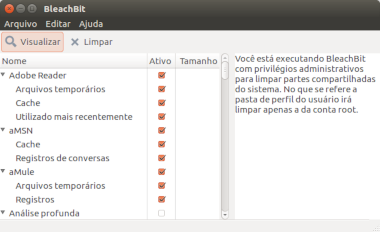
\includegraphics[width=0.9\linewidth]{cap04/Organiza/Bleachbit.png} 
 \end{wrapfigure}
  No Windows usava o CCleaner para limpar arquivos temporários, logs e muitas sujeiras deixadas pelo sistema. No Linux existem comandos de terminal para isso, mas prefiro usar um aplicativo gráfico que me permita fazer isso por aplicativo instalado e neste escolher o que desejo ou não remover, ou seja ter muito mais liberdade de escolha. Lembre-se sempre que quanto mais limpo seu sistema mais rápido realizará as operações.
\end{minipage}

\paragraph{Gramps – Árvore Genealógica}
\begin{minipage}{\linewidth}
 \vspace{5pt}
 \begin{wrapfigure}{l}{0.25\textwidth}
  \vspace{-\baselineskip}
  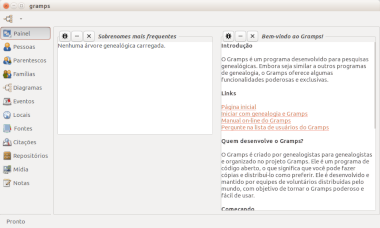
\includegraphics[width=0.9\linewidth]{cap04/Organiza/Gramps.png} 
 \end{wrapfigure}
 Já que estamos falando em Organização, que tal arrumarmos nossa família, não nada de programação ou Orientação a Objetos, estou falando de sabermos de onde viemos (e para onde vamos). Este é um aplicativo que seus netos poderão dar continuidade e entender qual sua origem e quem sabe agradecê-lo por isso. Aviso que a montagem de uma árvore familiar não é um trabalho fácil mas no final das contas pode ser bem prazeroso. Instalação Via Terminal.
\end{minipage}

\paragraph{KMyMoney – Gerenciador Financeiro}
\begin{minipage}{\linewidth}
 \vspace{5pt}
 \begin{wrapfigure}{l}{0.25\textwidth}
  \vspace{-\baselineskip}
  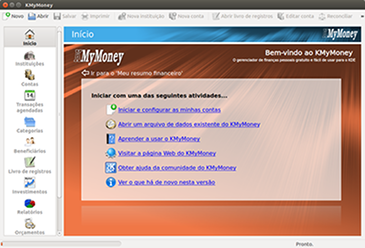
\includegraphics[width=0.9\linewidth]{cap04/Organiza/KMyMoney.png} 
 \end{wrapfigure}
 Que tal ter um assistente que pode lhe ajudar com as suas finanças. É possível incluir informações pessoais, seu banco, suas receitas correntes e diferentes categorias de despesas. E se não desejar inserir todas essas informações, pode pular tudo e se concentrar apenas na criação das categorias de receitas e despesas, bem como os diferentes tipos de contas (simplesmente rotulados como Dinheiro, Conta-corrente ou Poupança).
\end{minipage}

\paragraph{Nemo – Gerenciador de pastas}
\begin{minipage}{\linewidth}
 \vspace{5pt}
 \begin{wrapfigure}{l}{0.25\textwidth}
  \vspace{-\baselineskip}
  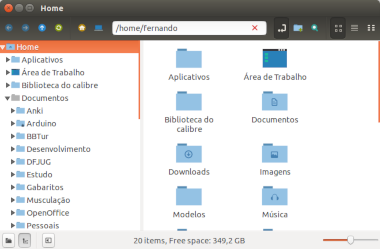
\includegraphics[width=0.9\linewidth]{cap04/Organiza/Nemo.png} 
 \end{wrapfigure}
 Não posso negar que o \textbf{Windows Explorer} vicia a gente a trabalhar de uma certa forma e ter que mudar essa forma não fazia parte dos meus planos, gosto do \textbf{Nautilus} mas o Nemo é muito mais semelhante, principalmente em se poder deixar uma hierarquia de árvores do lado esquerdo – Curioso que este é o Gerenciador de Pastas padrão do \textbf{Linux Mint}. A maior vantagem é não ser necessário se adaptar a um novo gerenciador de pastas.
\end{minipage}

\paragraph{Planner – Planejamento de Projetos}
\begin{minipage}{\linewidth}
 \vspace{5pt}
 \begin{wrapfigure}{l}{0.25\textwidth}
  \vspace{-\baselineskip}
  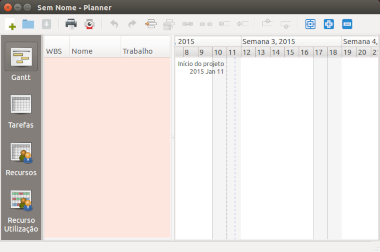
\includegraphics[width=0.9\linewidth]{cap04/Organiza/Planner.png} 
 \end{wrapfigure}
 Este é um daqueles aplicativos que não posso viver sem, junto ao MS-Office existe o \textbf{MS-Project} e foi um dos que mais senti falta quando o abandonei, deste modo corri atrás de um substituto e o Planner se encaixou como uma luva. Possui suporte ao gráfico de \textit{Gantt}, organização de tarefas e alocação de recursos. É totalmente gratuito e foi escrito um pequeno grupo de colaboradores que o mantém bem atualizado. Instalação Via Terminal.
\end{minipage}

\paragraph{SearchMonkey – Localizador de Documentos}
\begin{minipage}{\linewidth}
 \vspace{5pt}
 \begin{wrapfigure}{l}{0.25\textwidth}
  \vspace{-\baselineskip}
  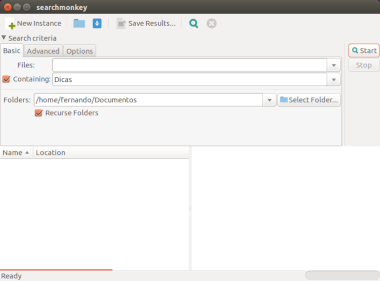
\includegraphics[width=0.9\linewidth]{cap04/Organiza/SearchMonkey.png} 
 \end{wrapfigure}
 As vezes localizar um determinado arquivo pode ser uma tarefa bem complicada, principalmente para pessoas que tem milhares deles perdidos em milhares de pastas. Esse aplicativo permite a pesquisa através de \textit{Expressões Regulares} para localizarmos um determinado arquivo. Podemos realizar a pesquisa por nomes ou conteúdos e isso permite que o ser muito mais preciso ao retornar os resultados. É possível localizar arquivos utilizando o comando \textbf{find} no terminal, mas pessoalmente prefiro o modo gráfico.
\end{minipage}

\paragraph{Tomboy – Organizador de Notas}
\begin{minipage}{\linewidth}
 \vspace{5pt}
 \begin{wrapfigure}{l}{0.25\textwidth}
  \vspace{-\baselineskip}
  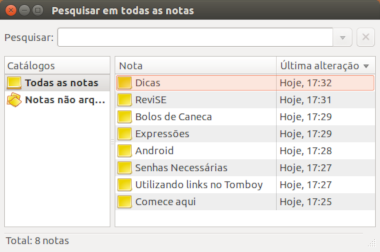
\includegraphics[width=0.9\linewidth]{cap04/Organiza/Tomboy.png} 
 \end{wrapfigure}
 No Windows peguei uma mania curiosa, criava um arquivo-texto com o bloco de notas e colocava na área de trabalho, eram dicas para me lembrar de algo como Expressões Regulares, Senhas ou mesmo receitas rápidas o problema é que ficava com a área de trabalho superpoluída, no Linux descobri este aplicativo para organizar tudo. É possível criar grupos para suas notas e terminar com aquele suplício de tentar achar aquela receita que viu na Web. 
\end{minipage}

\paragraph{wxBanker – Controle Pessoal de Contas}
\begin{minipage}{\linewidth}
 \vspace{5pt}
 \begin{wrapfigure}{l}{0.25\textwidth}
  \vspace{-\baselineskip}
  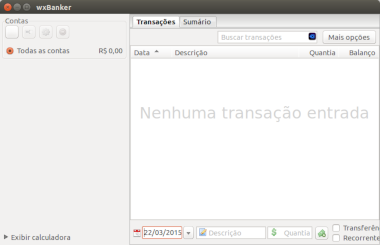
\includegraphics[width=0.9\linewidth]{cap04/Organiza/wxBanker.png}
 \end{wrapfigure}
 Qualquer empresário sabe que as contas da empresa não devem se misturar com as contas pessoais, mas como controlar essas contas? Esse aplicativo é a solução ideal, inúmeras contas e transações podem ser cadastradas e vários gráficos estão disponíveis para manter o controle de todas fácil e ainda poder contar com um belo saldo positivo no final do mês. Mas e o \textbf{KMyMoney}? Como disse, utilize o que preferir.
\end{minipage}

\section{Editores}\index{Biblioteca de Aplicativos}
Esses são os facilitadores de ações dentro de muitas áreas, tais como, um editor de textos mais potente que um simples bloco de notas mas não tão robusto quanto a um Writer (LibreOffice), para escrever um programa ou mesmo para uma troca com \textit{Expressões Regulares}.

Não gosta de expressões regulares e acha tudo isso uma frescura? Vamos então imaginar que possua um arquivo com um texto repleto de linhas em branco e queira eliminar todas, como fazer? Trocar uma por uma ou simplesmente usar uma expressão regular para realizar todo o serviço.

\paragraph{Atom – Editor de programação em diversas linguagens}
\begin{minipage}{\linewidth}
 \vspace{5pt}
 \begin{wrapfigure}{l}{0.25\textwidth}
  \vspace{-\baselineskip}
  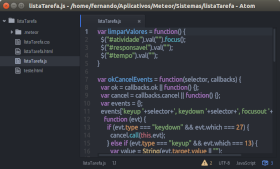
\includegraphics[width=0.9\linewidth]{cap04/Editores/Atom.png} 
 \end{wrapfigure}
 Quem vem do Mundo MacOS conhece o \textbf{Mate} um excelente editor para aplicações JavaScript.  O Atom se consolidou rapidamente por ser desenvolvido e consequentemente bem integrado ao padrão Git de versionamento. É um aplicativo open source, multiplataforma, leve e prático sua função básica é programação HTML, JavaScript (e suas vertentes) e o uso muito para Assembly, porém pode usado para qualquer linguagem. Instale o plugin \textbf{PlatformIO IDE Terminal} que permite acessar o terminal a partir do editor.
\end{minipage}

\paragraph{BlueJ – Editor para programação em linguagem Java}
\begin{minipage}{\linewidth}
 \vspace{5pt}
 \begin{wrapfigure}{l}{0.25\textwidth}
  \vspace{-\baselineskip}
  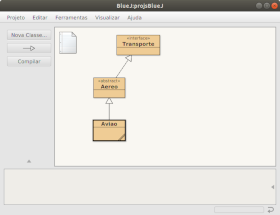
\includegraphics[width=0.9\linewidth]{cap04/Editores/Bluej.png} 
 \end{wrapfigure}
 Este é um dos eeditores mais leves que conheço para realizar coisas rápidas e práticas com a linguagem de programação Java. Torna-se ideal para estudantes ou aqueles que estão iniciando em Programação principalmente quando se trata em ensinar mapeamento de classes e Orientação a Objetos. Na nova versão vem ainda com o editor para Strider que é uma forma de se programar em blocos. Pacote .DEB no site: \url{http://www.bluej.org/}.
\end{minipage}

\paragraph{Code::Blocks IDE – Editor para programação em linguagem C++}
\begin{minipage}{\linewidth}
 \vspace{5pt}
 \begin{wrapfigure}{l}{0.25\textwidth}
  \vspace{-\baselineskip}
  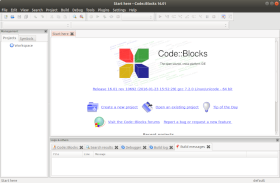
\includegraphics[width=0.9\linewidth]{cap04/Editores/Codeblocks.png} 
 \end{wrapfigure}
 Como bom programador Java torcia o nariz para C++, porém comecei a gostar da linguagem quando vi sua fácil integração com \textbf{Assembly} e passei a respeitá-la ainda mais quando fiz um curso de ``Jogos Digitais''. Acabei descobrindo uma linguagem bem versátil, apesar de ter seus limites, se encaixa muito bem nos meus planos de construir um jogo educacional. Porque não fazê-lo com Java ou Python? E cadê a graça do desafio?
\end{minipage}

\paragraph{Evolus Pencil – Prototipação de projetos}
\begin{minipage}{\linewidth}
 \vspace{5pt}
 \begin{wrapfigure}{l}{0.25\textwidth}
  \vspace{-\baselineskip}
  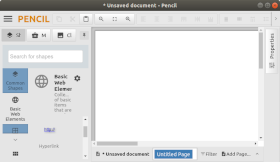
\includegraphics[width=0.9\linewidth]{cap04/Editores/Pencil.png} 
 \end{wrapfigure}
 Ter a mão uma ferramenta de prototipação ajuda na concepção de sistemas, como Analista não consigo me imaginar sem. Considero o Pencil o melhor aplicativo nessa categoria principalmente para projetos Web e Mobile, entretanto também me ajuda muito quando preciso mostrar um Fluxograma nas aulas. Pacote .DEB no site: \url{https://pencil.evolus.vn}.
\end{minipage}

\paragraph{Geany – Editor de textos com Expressões Regulares}
\begin{minipage}{\linewidth}
 \vspace{5pt}
 \begin{wrapfigure}{l}{0.25\textwidth}
  \vspace{-\baselineskip}
  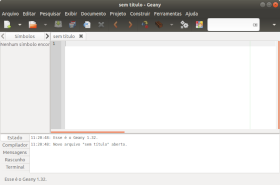
\includegraphics[width=0.9\linewidth]{cap04/Editores/Geany.png} 
 \end{wrapfigure}
 Não tenho absolutamente nada contra ao \textbf{gEdit} da mesma forma que não tenho com o \textbf{Bloco de Notas} e acredito que ambos aplicativos são úteis mas deixam a desejar no quesito quanto a pesquisa no texto com o uso de \textit{Expressões Regulares}. O único que se compara a este editor é o \textbf{Notepad++} porém mesmo com sua vinda ao mundo Linux (pode encontrá-lo na Loja) ainda prefiro usar o Geany que me quebrou muitos galhos.
\end{minipage}

\paragraph{Greenfoot – Editor para Aprendizado de Java}
\begin{minipage}{\linewidth}
 \vspace{5pt}
 \begin{wrapfigure}{l}{0.25\textwidth}
  \vspace{-\baselineskip}
  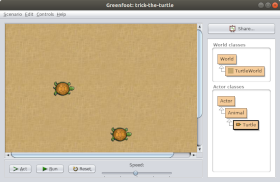
\includegraphics[width=0.9\linewidth]{cap04/Editores/Greenfoot.png} 
 \end{wrapfigure}
 Este projeto foi criado pelo \textit{King's College London} para o ensino e difusão da linguagem de programação Java, voltado para crianças e iniciantes. É o editor ideal para o iniciante, mas descobri uma forma muito fácil de criar jogos em Java. Seu editor é um caso a parte pois a programação é realizada em blocos. Pacote .DEB no site: \url{https://www.greenfoot.org}.
\end{minipage}

\paragraph{IntelliJ IDEA Community – Editor para programação em linguagem Java}
\begin{minipage}{\linewidth}
 \vspace{5pt}
 \begin{wrapfigure}{l}{0.25\textwidth}
  \vspace{-\baselineskip}
  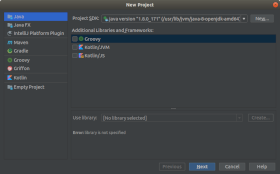
\includegraphics[width=0.9\linewidth]{cap04/Editores/Idea.png} 
 \end{wrapfigure}
 Antigamente existia uma briga sobre qual era o melhor editor para Java. Não desejo neste livro convencer ninguém a nada, nem a usar o \textbf{Ubuntu} quero convencer, use-o por gosto não porque lhe disse para usar. Com editor é a mesma coisa, uso tanto o \textbf{Eclipse} quanto este, a diferença é que ele se integra melhor com linguagens como \textbf{Kotlin} e \textbf{Flutter}. Não conhece essas linguagens, recomendo correr e se atualizar.
\end{minipage}

\paragraph{TeXstudio – Editor para Latex}
\begin{minipage}{\linewidth}
 \vspace{5pt}
 \begin{wrapfigure}{l}{0.25\textwidth}
  \vspace{-\baselineskip}
  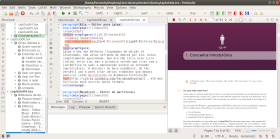
\includegraphics[width=0.9\linewidth]{cap04/Editores/TeXstudio.png} 
 \end{wrapfigure}
 Devo confessar que uma das mais importantes escolhas de uma linguagem é seu editor, usava o \textbf{Kile} até descobrir este. Este livro por exemplo é composto de vários arquivos (ficaria enorme em apenas um) e no TeXstudio fica muito mais simples realizar esta tarefa, além de vários atalhos práticos.
\end{minipage}

\paragraph{MuseScore – Editor de partituras}
\begin{minipage}{\linewidth}
 \vspace{5pt}
 \begin{wrapfigure}{l}{0.25\textwidth}
  \vspace{-\baselineskip}
  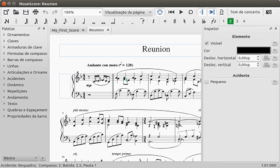
\includegraphics[width=0.9\linewidth]{cap04/Editores/Musescore.png} 
 \end{wrapfigure}
 É curioso como as pessoas da área de informática normalmente possuem como hobby tocar algum instrumento – não pretendo ser nenhuma exceção. No Linux não conheço nada melhor que este aplicativo para realizar o trabalho, além de criar e editar partituras ainda permite transformá-las para arquivos em formato MIDI ou gerar um PDF para distribuição.
\end{minipage}

\paragraph{PDFSam – Unir e separar arquivos PDF}
\begin{minipage}{\linewidth}
 \vspace{5pt}
 \begin{wrapfigure}{l}{0.25\textwidth}
  \vspace{-\baselineskip}
  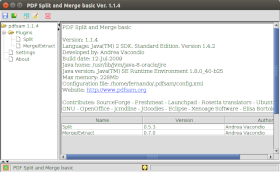
\includegraphics[width=0.9\linewidth]{cap04/Editores/PDFSam.png} 
 \end{wrapfigure}
 Este não é um leitor de PDF, serve para separá-los (Split) em vários arquivos ou juntá-los (Merge) em um único. Isso pode ser muito útil quando baixamos apostilas que vem em vários arquivos separados e desejamos ter um único arquivo, ou mesmo quando temos um PDF gigante mas só queremos determinadas folhas para entregar aos alunos. Lembre-se de possuir um backup do original.
\end{minipage}

\paragraph{PyCharm CE – Editor para programação em linguagem Python}
\begin{minipage}{\linewidth}
 \vspace{5pt}
 \begin{wrapfigure}{l}{0.25\textwidth}
  \vspace{-\baselineskip}
  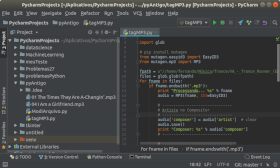
\includegraphics[width=0.9\linewidth]{cap04/Editores/Pycharm.png} 
 \end{wrapfigure}
 Python é uma linguagem espetacular, o Linux a torna seu par perfeito. Este editor foi desenvolvido pela JetBrains e é considerado um dos melhores, existe a versão Professional, mas pessoalmente prefiro esta. Oferece todo o suporte que preciso para programar com Python, além de um autocomplete de códigos fechando com uma boa comunicação com o ambiente \textbf{Git}.
\end{minipage}

\paragraph{RStudio – Editor para programação em linguagem R}
\begin{minipage}{\linewidth}
 \vspace{5pt}
 \begin{wrapfigure}{l}{0.25\textwidth}
  \vspace{-\baselineskip}
  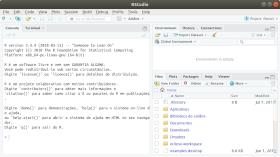
\includegraphics[width=0.9\linewidth]{cap04/Editores/RStudio.png} 
 \end{wrapfigure}
 R não é uma linguagem nova, porém a \textit{Data Science} (ou Ciência de Dados) só teve sua explosão a partir deste ano. Não vou entrar no detalhe que existe uma briga se é melhor usar Python ou R, o que sei é que desejo dominar ambas as linguagens e me tornar o mais empregável possível. Esta linguagem é baseada fortemente em Pacotes (do tipo quanto mais melhor) e funções.
\end{minipage}

\paragraph{Scribus – Editoração de textos}
\begin{minipage}{\linewidth}
 \vspace{5pt}
 \begin{wrapfigure}{l}{0.25\textwidth}
  \vspace{-\baselineskip}
  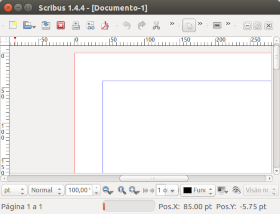
\includegraphics[width=0.9\linewidth]{cap04/Editores/Scribus.png} 
 \end{wrapfigure}
 É possível sem o menor problema utilizar o LibreOffice para realizar a editoração de uma revista, mas garanto que com este aplicativo o resultado final se torna muito mais interessante. Basta um pouco de pesquisa para comprovar que a grande maioria das revistas livres são produzidas com este software. Quando resolvi criar a ReviSE\footnote{Em: \url{http://fernandoanselmo.orgfree.com/wordpress/?page_id=173}} não tive a menor dúvida qual editor escolher para o trabalho e garanto que não me decepcionei, só pode ser comparado aqueles produtos da Adobe.
\end{minipage}

\paragraph{Sweet Home 3D – Editor de design de interior}
\begin{minipage}{\linewidth}
 \vspace{5pt}
 \begin{wrapfigure}{l}{0.25\textwidth}
  \vspace{-\baselineskip}
  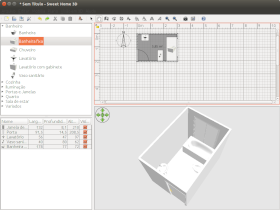
\includegraphics[width=0.9\linewidth]{cap04/Editores/Sweet.png} 
 \end{wrapfigure}
 Gosta de ficar mudando os móveis de lugar? Este é o aplicativo ideal, leve e completo, possui diversas opções de mobiliário. Construa a planta, levante as paredes, crie os cômodos, coloque as portas, as janelas e por fim o mobiliário, o ideal é ter a planta baixa do imóvel. Enquanto faz tudo em 2D (na planta baixa) o aplicativo recria tudo em uma visão 3D. A grande vantagem é que sempre teremos a mão uma planta baixa da casa e quando resolver arrumar a cozinha, pode tirar uma onda de arquiteto.
\end{minipage}

\section{Internet}\index{Biblioteca de Aplicativos}
Hoje em dia é impossível não estar conectado ao mundo virtual, por mais que se queira ficar em um sítio afastado de toda a tecnologia apenas curtindo o som dos pássaros e dos grilos noturnos, não tem jeito a Internet é um mal necessário assim como alguns aplicativos.\\[3mm]
Não espere encontrar muita coisa aqui, os programas padrões \textbf{Firefox}, \textbf{Remmina}, \textbf{Thunderbird} e \textbf{Transmission} já suprem boa parte do meu desejo de navegação, só preciso complementá-los.

\paragraph{DropBox – Armazenamento de arquivos}
\begin{minipage}{\linewidth}
 \vspace{5pt}
 \begin{wrapfigure}{l}{0.25\textwidth}
  \vspace{-\baselineskip}
  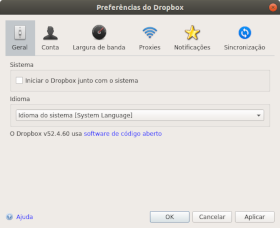
\includegraphics[width=0.9\linewidth]{cap04/Internet/Dropbox.png} 
 \end{wrapfigure}
 Com o advento do armazenamento na nuvem o Dropbox se tornou um dos programas mais usados (acho que pareia muito bem com o \textbf{Git}). Ao usar este programa, nunca mais tive medo de formatar o computador ou perder algo. Meus principais arquivos estão em um disco externo ou armazenados aqui. Ao baixar o aplicativo da Loja, parece que nada foi instalado, repare na barra superior seu ícone e observe que no \textbf{Nautilus} existe uma pasta de acesso para o Dropbox.
\end{minipage}

\paragraph{FileZilla – Transferência de dados via FTP}
\begin{minipage}{\linewidth}
 \vspace{5pt}
 \begin{wrapfigure}{l}{0.25\textwidth}
  \vspace{-\baselineskip}
  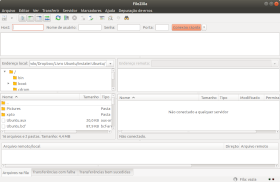
\includegraphics[width=0.9\linewidth]{cap04/Internet/Filezilla.png} 
 \end{wrapfigure}
 Para aqueles que possuem um site, sabem como é impossível ficar sem um cliente \textbf{FTP} para a transferência de arquivos. Este é melhor aplicativo nessa categoria, prático, rápido e muito fácil de usar. Basta apenas se conectar e arrastar os arquivos do endereço local para o endereço remoto. Acho que foi um dos poucos clientes FTP que nunca tive o menor aborrecimento e sempre me atendeu no que foi preciso.
\end{minipage}

\paragraph{Liferea – Agregador de notícias}
\begin{minipage}{\linewidth}
 \vspace{5pt}
 \begin{wrapfigure}{l}{0.25\textwidth}
  \vspace{-\baselineskip}
  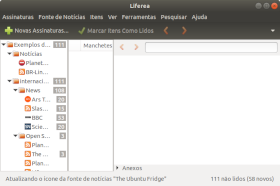
\includegraphics[width=0.9\linewidth]{cap04/Internet/Liferea.png} 
 \end{wrapfigure}
 O Liferea, abreviatura para \textit{Linux Feed Reader}, é um excelente leitor/agregador de notícias e que reúne todo o conteúdo de seus blogs favoritos em uma interface simples que faz com que seja fácil de organizar e pesquisar feeds (procurar no blog um link para \textbf{RSS}). Para adicionar um Blog pressione o botão ``Novas Assinaturas...'', cole o endereço RSS\footnote{O meu é: \url{http://fernandoanselmo.blogspot.com/feeds/posts/default}} e assim será avisado quando uma nova publicação for postada.
\end{minipage}

\paragraph{Postman – Envio de informações REST}
\begin{minipage}{\linewidth}
 \vspace{5pt}
 \begin{wrapfigure}{l}{0.25\textwidth}
  \vspace{-\baselineskip}
  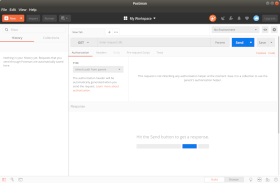
\includegraphics[width=0.9\linewidth]{cap04/Internet/Postman.png} 
 \end{wrapfigure}
 Precisa testar uma chamada e o site pede um método POST, só tem duas coisas a fazer ou construir um formulário em HTML ou usar este aplicativo. É um dos melhores que conheço pois aceita enviar todo o tipo de arquivo conhecido bem como recebê-los. Postman evoluiu tanto que agora é possível salvar e compartilhar os testes realizados.
\end{minipage}

\section{Jogos}\index{Biblioteca de Aplicativos}
Fiquei na dúvida se colocaria ou não essa seção neste livro, acredito que cada pessoa tenha sua preferência em relação aos jogos, porém quis mostrar que o Linux também pode ser usado para diversão. Só que irei me limitar aos jogos encontrados diretamente na loja e considerados úteis combatentes do estresse.

Mas se realmente deseja jogos de ação mais profissionais, recomendo baixar o \textbf{Steam for Linux}. Foi criado pela \textit{Valve} (mesma empresa que criou entre outros sucessos o \textbf{Counter Strike}) como uma plataforma para a distribuição de conteúdos digitais. E se gosta de simuladores (MSX, NES, Game Boy e outros) pesquise na loja por: \textit{Emulator}, encontrará muitos a disposição.

\paragraph{0 A.D. – Jogo de estratégia}
\begin{minipage}{\linewidth}
 \vspace{5pt}
 \begin{wrapfigure}{l}{0.25\textwidth}
  \vspace{-\baselineskip}
  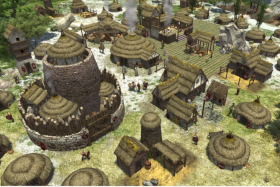
\includegraphics[width=0.9\linewidth]{cap04/Jogos/0ad.png} 
 \end{wrapfigure}
 Quer baixar o Stress rapidamente? Que tal viver como Romano, Espartano ou alguma outra civilização antiga. 0 A.D. (pronuncia ``zero ey-dee'') é um jogo com base em conceitos históricos de Economia, Guerra e Religião das antigas civilizações, ainda está sendo construído, mas o que já existe dá show. Acredito que a única comparação que consigo fazer é com \textit{Civilization}, o visual é incrível e as músicas recomendo baixar todas no site oficial.
\end{minipage}

\paragraph{BurgerSpace – Desafio tipo arcade}
\begin{minipage}{\linewidth}
 \vspace{5pt}
 \begin{wrapfigure}{l}{0.25\textwidth}
  \vspace{-\baselineskip}
  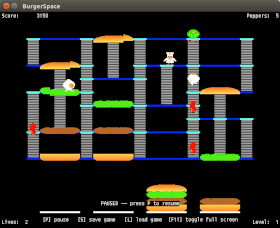
\includegraphics[width=0.9\linewidth]{cap04/Jogos/Burgerspace.png} 
 \end{wrapfigure}
 Conhecia este jogo por outro nome e nada tem a ver com Espaço, só o divertimento que continua o mesmo, sua missão é completar os hambúrgueres enquanto foge de salsichas, ovos e picles assassinos (é possível derrubá-los junto com os hambúrgueres e assim ganhar mais pontos), lá na minha época do Windows/DOS foi um dos primeiros jogos que conheci (ainda num terminal com tela verde) é divertimento equivalente a ``Elevator Action'', me lembra muito as antigas máquinas de fliperama.
\end{minipage}

\paragraph{Chromium B.S.U. – Jogo de tiro espacial}
\begin{minipage}{\linewidth}
 \vspace{5pt}
 \begin{wrapfigure}{l}{0.25\textwidth}
  \vspace{-\baselineskip}
  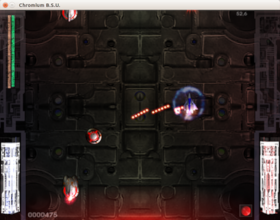
\includegraphics[width=0.9\linewidth]{cap04/Jogos/ChromiumBSU.png} 
 \end{wrapfigure}
 Não confunda esse Jogo com o navegador. Este é um jogo para quando sua carga de Stress estiver muito alta e deseja descarregar matando tudo sem parar. Pegue as caveiras e os Tux que vão descendo na tela para ter mais poder de fogo, ampliar seu escudo de força e assim sobreviver ao ataque das naves, só uma dica: seja bem rápido. Se está com raiva de alguém ou alguma coisa esse jogo torna-se um ótimo anti estressante para ajudá-lo a esfriar a cabeça, só não vale ficar mais irritado ainda por perder.
\end{minipage}

\paragraph{Super Tux 2 – Jogo no estilo de plataforma 2D}
\begin{minipage}{\linewidth}
 \vspace{5pt}
 \begin{wrapfigure}{l}{0.25\textwidth}
  \vspace{-\baselineskip}
  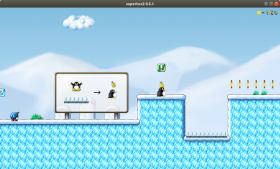
\includegraphics[width=0.9\linewidth]{cap04/Jogos/supertux.png} 
 \end{wrapfigure}
 Sente falta de saltar obstáculos com o Mario ou da velocidade do Sonic? Não se preocupe esse jogo vai fazer esquecê-los rapidinho, no mesmo estilo dos melhores jogos 2D percorra várias trilhas, pule sobre seus inimigos, colecione moedas e vários prêmios que estão escondidos nos 26 níveis para serem concluídos e assim salvarmos \textit{Penny} a namorada do \textit{Tux}.
\end{minipage}

\paragraph{SuperTuxKart – Corrida no estilo Mario Kart}
\begin{minipage}{\linewidth}
 \vspace{5pt}
 \begin{wrapfigure}{l}{0.25\textwidth}
  \vspace{-\baselineskip}
  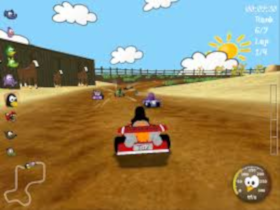
\includegraphics[width=0.9\linewidth]{cap04/Jogos/supertuxkart.png} 
 \end{wrapfigure}
 Esse um dos mais divertido jogos 3D com personagens que representam os softwares do mundo livre, então além do próprio \textit{Tux} temos o \textit{Wilber} (Gimp), o \textit{Konqi} (KDE) e muitos outros. São várias pistas que são desbloqueadas a medida que sua experiência vai aumentando e com cenários engraçados é a diversão garantida para os mais estressados. No jogo além de poder jogar as corridas em modo separado ainda é possível cumprir uma história e livrar o mundo do Software Livre sobre um grande perigo que caiu.
\end{minipage}

\paragraph{Tali – Jogo de dados}
\begin{minipage}{\linewidth}
 \vspace{5pt}
 \begin{wrapfigure}{l}{0.25\textwidth}
  \vspace{-\baselineskip}
  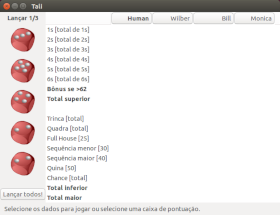
\includegraphics[width=0.9\linewidth]{cap04/Jogos/Tali.png} 
 \end{wrapfigure}
 Tali é uma mistura de sorte, jogo de Poker e estratégia, conta a lenda que sua origem remonta dos exércitos romanos que utilizavam o jogo como diversão, cinco dados são jogados e devemos selecionar a opção que mais permite pontuar, só que são 13 opções e 13 jogadas dos dados. Provavelmente no começo achará esse jogo bobo mas com a possibilidade de jogar em rede contra os colegas do trabalho torna-o muito divertido.
\end{minipage}

\paragraph{Extreme Tux Racer – Corrida de Velocidade}
\begin{minipage}{\linewidth}
 \vspace{5pt}
 \begin{wrapfigure}{l}{0.25\textwidth}
  \vspace{-\baselineskip}
  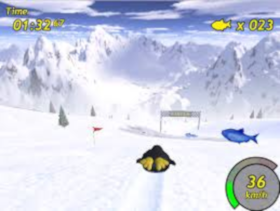
\includegraphics[width=0.9\linewidth]{cap04/Jogos/ExtremeTuxRacer.png} 
 \end{wrapfigure}
 Presente por padrão em várias distribuições voltadas para crianças, é um divertido jogo 3D para todos aqueles que desejam descer uma montanha a toda velocidade, no meio do caminho pegar o maior número de peixes e ainda fazer no menor tempo possível. A única dica que posso dar é tome cuidado para não ficar preso pois durante o jogo existem algumas armadilha que é impossível sair do lugar, além disso é excelente para chamar todo mundo da família para ver quem consegue chegar na linha de chegada.
\end{minipage}

\paragraph{XBoard – Jogo de Xadrez}
\begin{minipage}{\linewidth}
 \vspace{5pt}
 \begin{wrapfigure}{l}{0.25\textwidth}
  \vspace{-\baselineskip}
  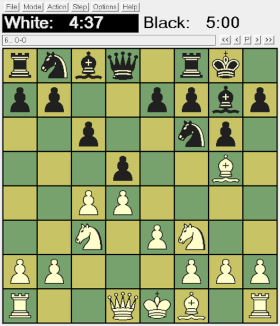
\includegraphics[width=0.9\linewidth]{cap04/Jogos/XBoard.png} 
 \end{wrapfigure}
 Me tire todos meus jogos mas deixe meu tabuleiro de Xadrez e esse aqui é realmente impressionante, como as partidas que fazia com meu pai. Se conseguir ganhar do computador no modo mais difícil já pode começar a pensar em seguir uma nova carreira. Só que não para por aí, este programa pode ser usado como um Servidor de Xadrez para jogos em rede ou que tal uma partida por e-mail, além de gráficos e uma porção de dados estatísticos para que possa desenvolver uma melhor partida na próxima. Curiosidade, existia um livro que queria escrever e se chamaria ``Xadrez em Java'', tinha alguns capítulos pronto mas o destino não quis que o terminasse.
\end{minipage}

\paragraph{XGalaga++ – Desafio tipo arcade}
\begin{minipage}{\linewidth}
 \vspace{5pt}
 \begin{wrapfigure}{l}{0.25\textwidth}
  \vspace{-\baselineskip}
  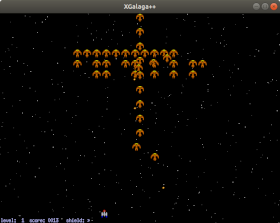
\includegraphics[width=0.9\linewidth]{cap04/Jogos/xgalaga.png} 
 \end{wrapfigure}
 Um jogo que gastei muito, mas muito mesmo (foram mesadas inteiras) no fliperama foi \textbf{Galaga}, pois este jogo vicia. Uma nave deve cruzar o universo e para conseguir isso deve acabar com hordas de naves invasoras que partem para ataques suicidas, só existe uma única saída ser tão louco quanto os alienígenas. Lembro de uma vez no fliperama criaram um campeonato, existia um garoto que era excelente, fui desafiá-lo e... não cheguei nem perto do score que ele fez (histórias que o Nerd se dá bem só acontece em filmes). Uma boa alternativa é baixar também o pacote Snap do jogo conhecido por \textbf{JGalaxian} através do seguinte comando no terminal: snap install jgalaxian
\end{minipage}

\section{Imagem, Som e Vídeo}\index{Biblioteca de Aplicativos}
Ter um computador significa que vamos manipular imagens (muitas), ouvir músicas (muitas) e assistir vídeos (muitos), tudo isso tem um alto custo de armazenamento ou banda de rede mas vale a pena. Afinal para que serve o computador senão como uma ferramenta para nos divertirmos? Vamos em frente pois é a seção que mais uso.

\paragraph{Audacious – Reprodutor de MP3}
\begin{minipage}{\linewidth}
 \vspace{5pt}
 \begin{wrapfigure}{l}{0.25\textwidth}
  \vspace{-\baselineskip}
  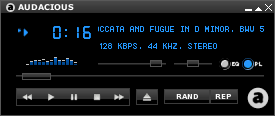
\includegraphics[width=0.9\linewidth]{cap04/Som/Audacious.png} 
 \end{wrapfigure}
 Muitas pessoas, me incluo nessa lista, adoravam o \textbf{WinAMP}, durante muito tempo foi um dos principais reprodutores de música no Windows. O \textbf{Rhythmbox} é excelente mas tem um problema quanto a simplicidade ou mesmo em recordar em qual música de uma lista paramos e isso é terrível quando se deseja ouvir um ``Áudio Livro''.
\end{minipage}

\paragraph{Audacity – Editar trilhas de áudio}
\begin{minipage}{\linewidth}
 \vspace{5pt}
 \begin{wrapfigure}{l}{0.25\textwidth}
  \vspace{-\baselineskip}
  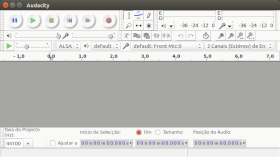
\includegraphics[width=0.9\linewidth]{cap04/Som/Audacity.png} 
 \end{wrapfigure}
 Acabou de baixar uma trilha de áudio para compor um software ou uma apresentação, mas deseja apenas um pedaço, realizar determinados cortes ou mesmo adicionar partes de um outro áudio este é o editor que pode lhe ajudar a fazer tudo isso e muito mais. Uma das coisas mais interessantes que é possível fazer é eliminar as vozes das músicas e assim conseguir um excelente arquivo para aquele animado Karaokê.
\end{minipage}

\paragraph{Easytag – Manipular tags de MP3}
\begin{minipage}{\linewidth}
 \vspace{5pt}
 \begin{wrapfigure}{l}{0.25\textwidth}
  \vspace{-\baselineskip}
  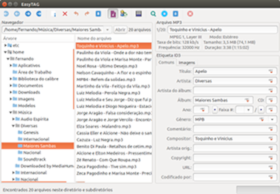
\includegraphics[width=0.9\linewidth]{cap04/Som/Easytag.png} 
 \end{wrapfigure}
 Possuir uma coleção de músicas em MP3 é a coisa mais fácil do mundo para qualquer usuário, porém mantê-la ordenada é um verdadeiro problema, este pequeno aplicativo auxilia nesse ponto. Permite rapidamente trocar os dados da etiqueta de vários arquivos simultaneamente, e padronizar o artista, álbum, ano e outros dados que seria uma tarefa bem maçante. Sua única desvantagem é que não é possível passar informação de uma tag por outra.
\end{minipage}

\paragraph{mp3splt-gtk audio splitter – Divisor de áudio}
\begin{minipage}{\linewidth}
 \vspace{5pt}
 \begin{wrapfigure}{l}{0.25\textwidth}
  \vspace{-\baselineskip}
  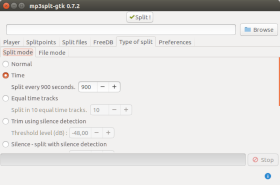
\includegraphics[width=0.9\linewidth]{cap04/Som/mp3splt.png} 
 \end{wrapfigure}
 O nome deste programa pode ser muito complicado, mas em compensação é muito prático, porém existem muitas opções para dividir um arquivo de áudio. A mais prática delas é acessar a aba \textbf{Type of split}, selecionar a opção \textbf{type}, digitar o tempo desejado (em segundos) e apertar o botão \textbf{Split}. Também é possível configurar para que os tempos de silêncio sejam automaticamente detectados e a divisão realizada.
\end{minipage}

\paragraph{MyPaint – Manipulação de Imagens}
\begin{minipage}{\linewidth}
 \vspace{5pt}
 \begin{wrapfigure}{l}{0.25\textwidth}
  \vspace{-\baselineskip}
  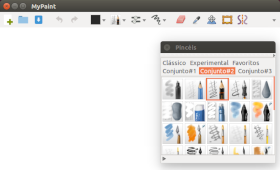
\includegraphics[width=0.9\linewidth]{cap04/Editores/Mypaint.png} 
 \end{wrapfigure}
 Não tenho absolutamente nada contra ao \textbf{Gimp}, muito pelo contrário, porém possuo uma mesa de desenho e prefiro usar o \textbf{MyPaint} que capta muito melhor a sensibilidade da caneta bem como me fornecer várias opções de estilos. Muitas vezes utilizo este aplicativo para iniciar um desenho que concluo no Gimp. A variedade de pínceis disponíveis neste editor supre todas minhas necessidades artísticas.
\end{minipage}

\paragraph{Pinta – Manipulação de Imagens}
\begin{minipage}{\linewidth}
 \vspace{5pt}
 \begin{wrapfigure}{l}{0.25\textwidth}
  \vspace{-\baselineskip}
  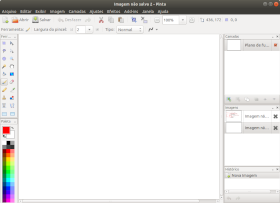
\includegraphics[width=0.9\linewidth]{cap04/Som/Pinta.png} 
 \end{wrapfigure}
 Comparativo do Pinta seria o mesmo que o antigo \textbf{MS-Paint}. É um dos mais práticos manipuladores de imagem que conheço tirando que mesmo com experiência zero em edição, ainda assim conseguir um excelente resultado. É ideal quando queremos apenas dar um retoque rápido em alguma imagem, selecionar uma área ou mesmo brincar de pintura. Utilizo principalmente para é criar MEMEs para publicar nas redes sociais.
\end{minipage}

\paragraph{SMPlayer – Reprodutor de vídeo}
\begin{minipage}{\linewidth}
 \vspace{5pt}
 \begin{wrapfigure}{l}{0.25\textwidth}
  \vspace{-\baselineskip}
  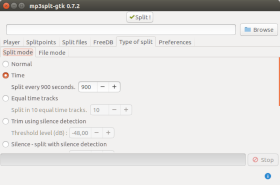
\includegraphics[width=0.9\linewidth]{cap04/Som/mp3splt.png} 
 \end{wrapfigure}
 O \textbf{Totem} é um excelente reprodutor de vídeo porém existem algumas lacunas a serem preenchidas tal como buscar uma legenda automaticamente e alguns outros detalhes. SMPlayer é excelente e possui um enorme suporte a CODECS, além de suporte para vídeos do \textbf{YouTube}. Outro detalhe muito útil desse programa é a sua memória com a possibilidade de recordar exatamente onde parou o vídeo.
\end{minipage}

\paragraph{StopMotion – Criador de animações}
\begin{minipage}{\linewidth}
 \vspace{5pt}
 \begin{wrapfigure}{l}{0.25\textwidth}
  \vspace{-\baselineskip}
  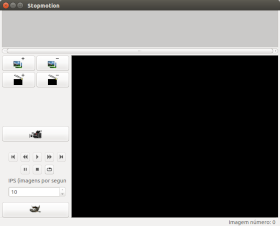
\includegraphics[width=0.9\linewidth]{cap04/Som/Stopmotion.png} 
 \end{wrapfigure}
 O primeiro filme tipo \textit{StopMotion} que vi na vida foi ``A Festa do Monstro Maluco'' (\textit{Mad Monster Party} – 1967), fiquei apaixonado por aqueles ``bonecos animados'' e sempre carreguei um sonho de produzi-los. Esse aplicativo permite importar imagens, adicionar efeitos sonoros e exportar a animação para diversos formatos. E quem sabe agora não realizo meu antigo sonho e me torno um produtor de filmes como \textbf{Tim Burton} e refaço ``Noiva Cadáver'' ou ``O Estranho Mundo de Jack''.
\end{minipage}

\paragraph{Synfig Studio – Animação de vetores 2D}
\begin{minipage}{\linewidth}
 \vspace{5pt}
 \begin{wrapfigure}{l}{0.25\textwidth}
  \vspace{-\baselineskip}
  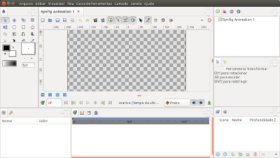
\includegraphics[width=0.9\linewidth]{cap04/Som/Synfig.png} 
 \end{wrapfigure}
 Synfig é a solução ideal para gerar animações 2D livre e de código aberto, foi criado com o intuito de criar um trabalho de boa qualidade cinematográfica usando vetores e mapa de bits, pode-se dizer que seu corrente mais forte é o \textbf{Blender}. Porém, aqui não existe a necessidade em se criar animações quadro a quadro.
\end{minipage}

\section{Estudo}\index{Biblioteca de Aplicativos}
Ter um computador e não utilizá-lo para estudo é como ter uma calculadora \textbf{HP 12C} e fazer apenas contas básicas. Não precisamos ser radicais e mudar para a distribuição \textbf{Edubuntu}, mas alguns aplicativos de ensino são fundamentais para se ter no computador. \\[3mm]
\begin{dica}[Professores ou Educadores] para muito mais aplicativos de estudo recomendo uma consulta a Tabela Dinâmica do Software Livre Educacional, disponível em \url{https://www.ufrgs.br/soft-livre-edu/wiki/Tabela_Dinâmica_Software_Educacional_livre}.
\end{dica}

\paragraph{Anki – Baralhos de flashcard}
\begin{minipage}{\linewidth}
 \vspace{5pt}
 \begin{wrapfigure}{l}{0.25\textwidth}
  \vspace{-\baselineskip}
  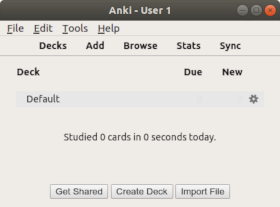
\includegraphics[width=0.9\linewidth]{cap04/Estudo/Anki.png} 
 \end{wrapfigure}
 Interessante método de estudo para provas que exigem decorar termos é criar baralhos de \textit{FlashCards} (cartões que de um lado possuem uma pergunta e de outro a resposta) que são possíveis de serem organizados por temas, assim estudar para uma certificação se torna uma tarefa um pouco mais simples. Este aplicativo possui uma versão para \textbf{Android} e os cartões podem ser compartilhados, tornando qualquer hora livre uma oportunidade de revisão.
\end{minipage}

\paragraph{Artha – Dicionário de Inglês}
\begin{minipage}{\linewidth}
 \vspace{5pt}
 \begin{wrapfigure}{l}{0.25\textwidth}
  \vspace{-\baselineskip}
  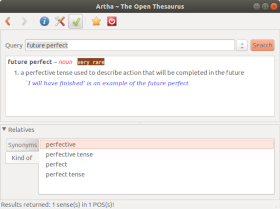
\includegraphics[width=0.9\linewidth]{cap04/Estudo/Artha.png} 
 \end{wrapfigure}
 \textit{I'm sorry, but knowledge Tio Sam's idiom is essential for everyone}. E quem nunca teve uma dúvida em alguma palavra que atire a primeira \textit{Slang}. Não pense que este é um dicionário simples, a ideia é que a comunidade ajude na sua construção então a medida que o tempo vai passando mais e mais palavras são adicionadas e ainda é acompanhada de frases exemplo. Em uma situação de aperto onde um grande dicionário está fora de alcance, este aplicativo pode ser uma tábua de salvação.
\end{minipage}

\paragraph{Calibre – Leitor de e-books}
\begin{minipage}{\linewidth}
 \vspace{5pt}
 \begin{wrapfigure}{l}{0.25\textwidth}
  \vspace{-\baselineskip}
  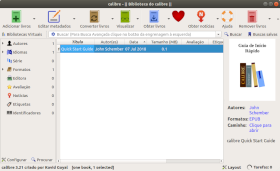
\includegraphics[width=0.9\linewidth]{cap04/Estudo/Calibre.png} 
 \end{wrapfigure}
 Os preços dos livros em papel são muito caros para um mero mortal, a saída é apelar para os livros digitais, este leitor permite não apenas a leitura como a organização de uma coleção de EPUB ou MOBI. Também possui um bom conjunto de recursos como facilitar a busca, a conversão para outros formatos e o Editor é instalado a parte, deste modo torna possível abrir este formato de arquivo com um duplo clique.
\end{minipage}

\paragraph{GeoGebra – Criar construções matemáticas dinâmicas}
\begin{minipage}{\linewidth}
 \vspace{5pt}
 \begin{wrapfigure}{l}{0.25\textwidth}
  \vspace{-\baselineskip}
  \includegraphics[width=0.9\linewidth]{cap04/Estudo/Geogebra.png} 
 \end{wrapfigure}
 Combina geometria, álgebra, tabelas, gráficos, estatística e cálculo em um único sistema com uma vantagem didática de apresentar, ao mesmo tempo, duas representações diferentes de um mesmo objeto contendo sua representação \textit{Geométrica} e sua representação \textit{Algébrica}. Também é possível inserir equações e coordenadas diretamente nos gráficos e possui todas as ferramentas tradicionais de um software de Geometria dinâmica: Pontos, Segmentos, Retas e Seções Cônicas.
\end{minipage}

\paragraph{GNU Octave – Expressões Matemáticas}
\begin{minipage}{\linewidth}
 \vspace{5pt}
 \begin{wrapfigure}{l}{0.25\textwidth}
  \vspace{-\baselineskip}
  \includegraphics[width=0.9\linewidth]{cap04/Estudo/GnuOctave.png} 
 \end{wrapfigure}
 No começo existia o \textbf{MathLab} porém era pago e dois professores da faculdade de Estatística resolveram criar um clone. O clone é tão parecido que até as funções são as mesmas, o objetivo de ambos professores era simplesmente permitir que seus alunos pudessem desfrutar do poder do MathLab sem ter que gastar para isso. Sua maior vantagem é poder usar (e aprender) qualquer tipo de expressão matemática, de matrizes a funções trigonométricas.
\end{minipage}

\paragraph{Tux Guitar – Aprendizado de Música}
\begin{minipage}{\linewidth}
 \vspace{5pt}
 \begin{wrapfigure}{l}{0.25\textwidth}
  \vspace{-\baselineskip}
  \includegraphics[width=0.9\linewidth]{cap04/Estudo/TuxGuitar.png} 
 \end{wrapfigure}
 Este programa facilmente conseguiria entrar em três seções: Editor de Partituras, Edição de Som MIDI mas preferi colocá-lo na seção de Estudo. O professor de música que desconhece esse, ou usa o \textbf{MuseScore} ou pagou uma nota por algum outro aplicativo com esse mesmo poder. É possível criar e tocar as partituras reproduzindo perfeitamente sons de vários instrumentos, além de poder salvar o resultado em arquivos de formato MIDI ou imprimir a partitura em PDF.
\end{minipage}

% Final do Capítulo
\clearpage